\chapter{Methodology}
\label{sec:methodology}
% \todo{Describe the design of our experiment. Break down experiment into sub experiments, how does that relate to the different subsystem we are building.}
% \todo{Describe the tools and processes we will use to validate our software. Nsight systems, nsight compute, other tools for measuring memory. Bash scripts for testing}
\section{Overview}
This thesis designs, implements, and evaluates a software-defined radar processing 
pipeline for a small monopulse radar system, assessing both computational efficiency 
and tracking accuracy on an NVIDIA Jetson Xavier NX and a Xavier AGX embedded GPU platform. 
The methodology is structured to directly address the gaps identified in the literature review: the
absence of radar algorithm performance evaluation in the noise regimes of air-to-air
small aperture radar, low level
implementation analysis, and hardware-aware design conclusions under SWaP constraints.
Through the methodology outlined in this chapter, we fulfill the contributions of this 
thesis, to compare radar algorithm configurations by sensitivity and track quality, to compare
low-level implementations by computational performance, and to derive hardware-aware design 
recommendations.

The software processing pipeline is designed to receive the radar data from multiple 
Texas Instruments 
AWR2243 radar chips, and produce tracks of targets in the radar's field of view. For 
the experiments performed in this work, we utilise data from a conformal synthetic 
aperture radar. Both the radar hardware and the software are designed to be modular. 
The radar module, depicted in Figure \ref{fig:radar-module},
has up to 12 receiver patches that are arranged in a 6x2 grid, conforming to a curved surface.
For testability, the software system is broken up into three subsystems, which are in turn 
comprised of stages that each perform a specific radar processing function. 
The three subsystems are: a pre-processing subsystem which is concerned with preparing 
the raw radar data for detection, an aggregator subsystem, which is concerned with combining the 
processed data from multiple video streams into a single stream, and a detection and tracking 
subsystem, which is concerned with detecting targets in the radar data and tracking them over time. 
This subsystem level design is depicted in Figure \ref{fig:system-level-dataflow}. 

\begin{figure}
    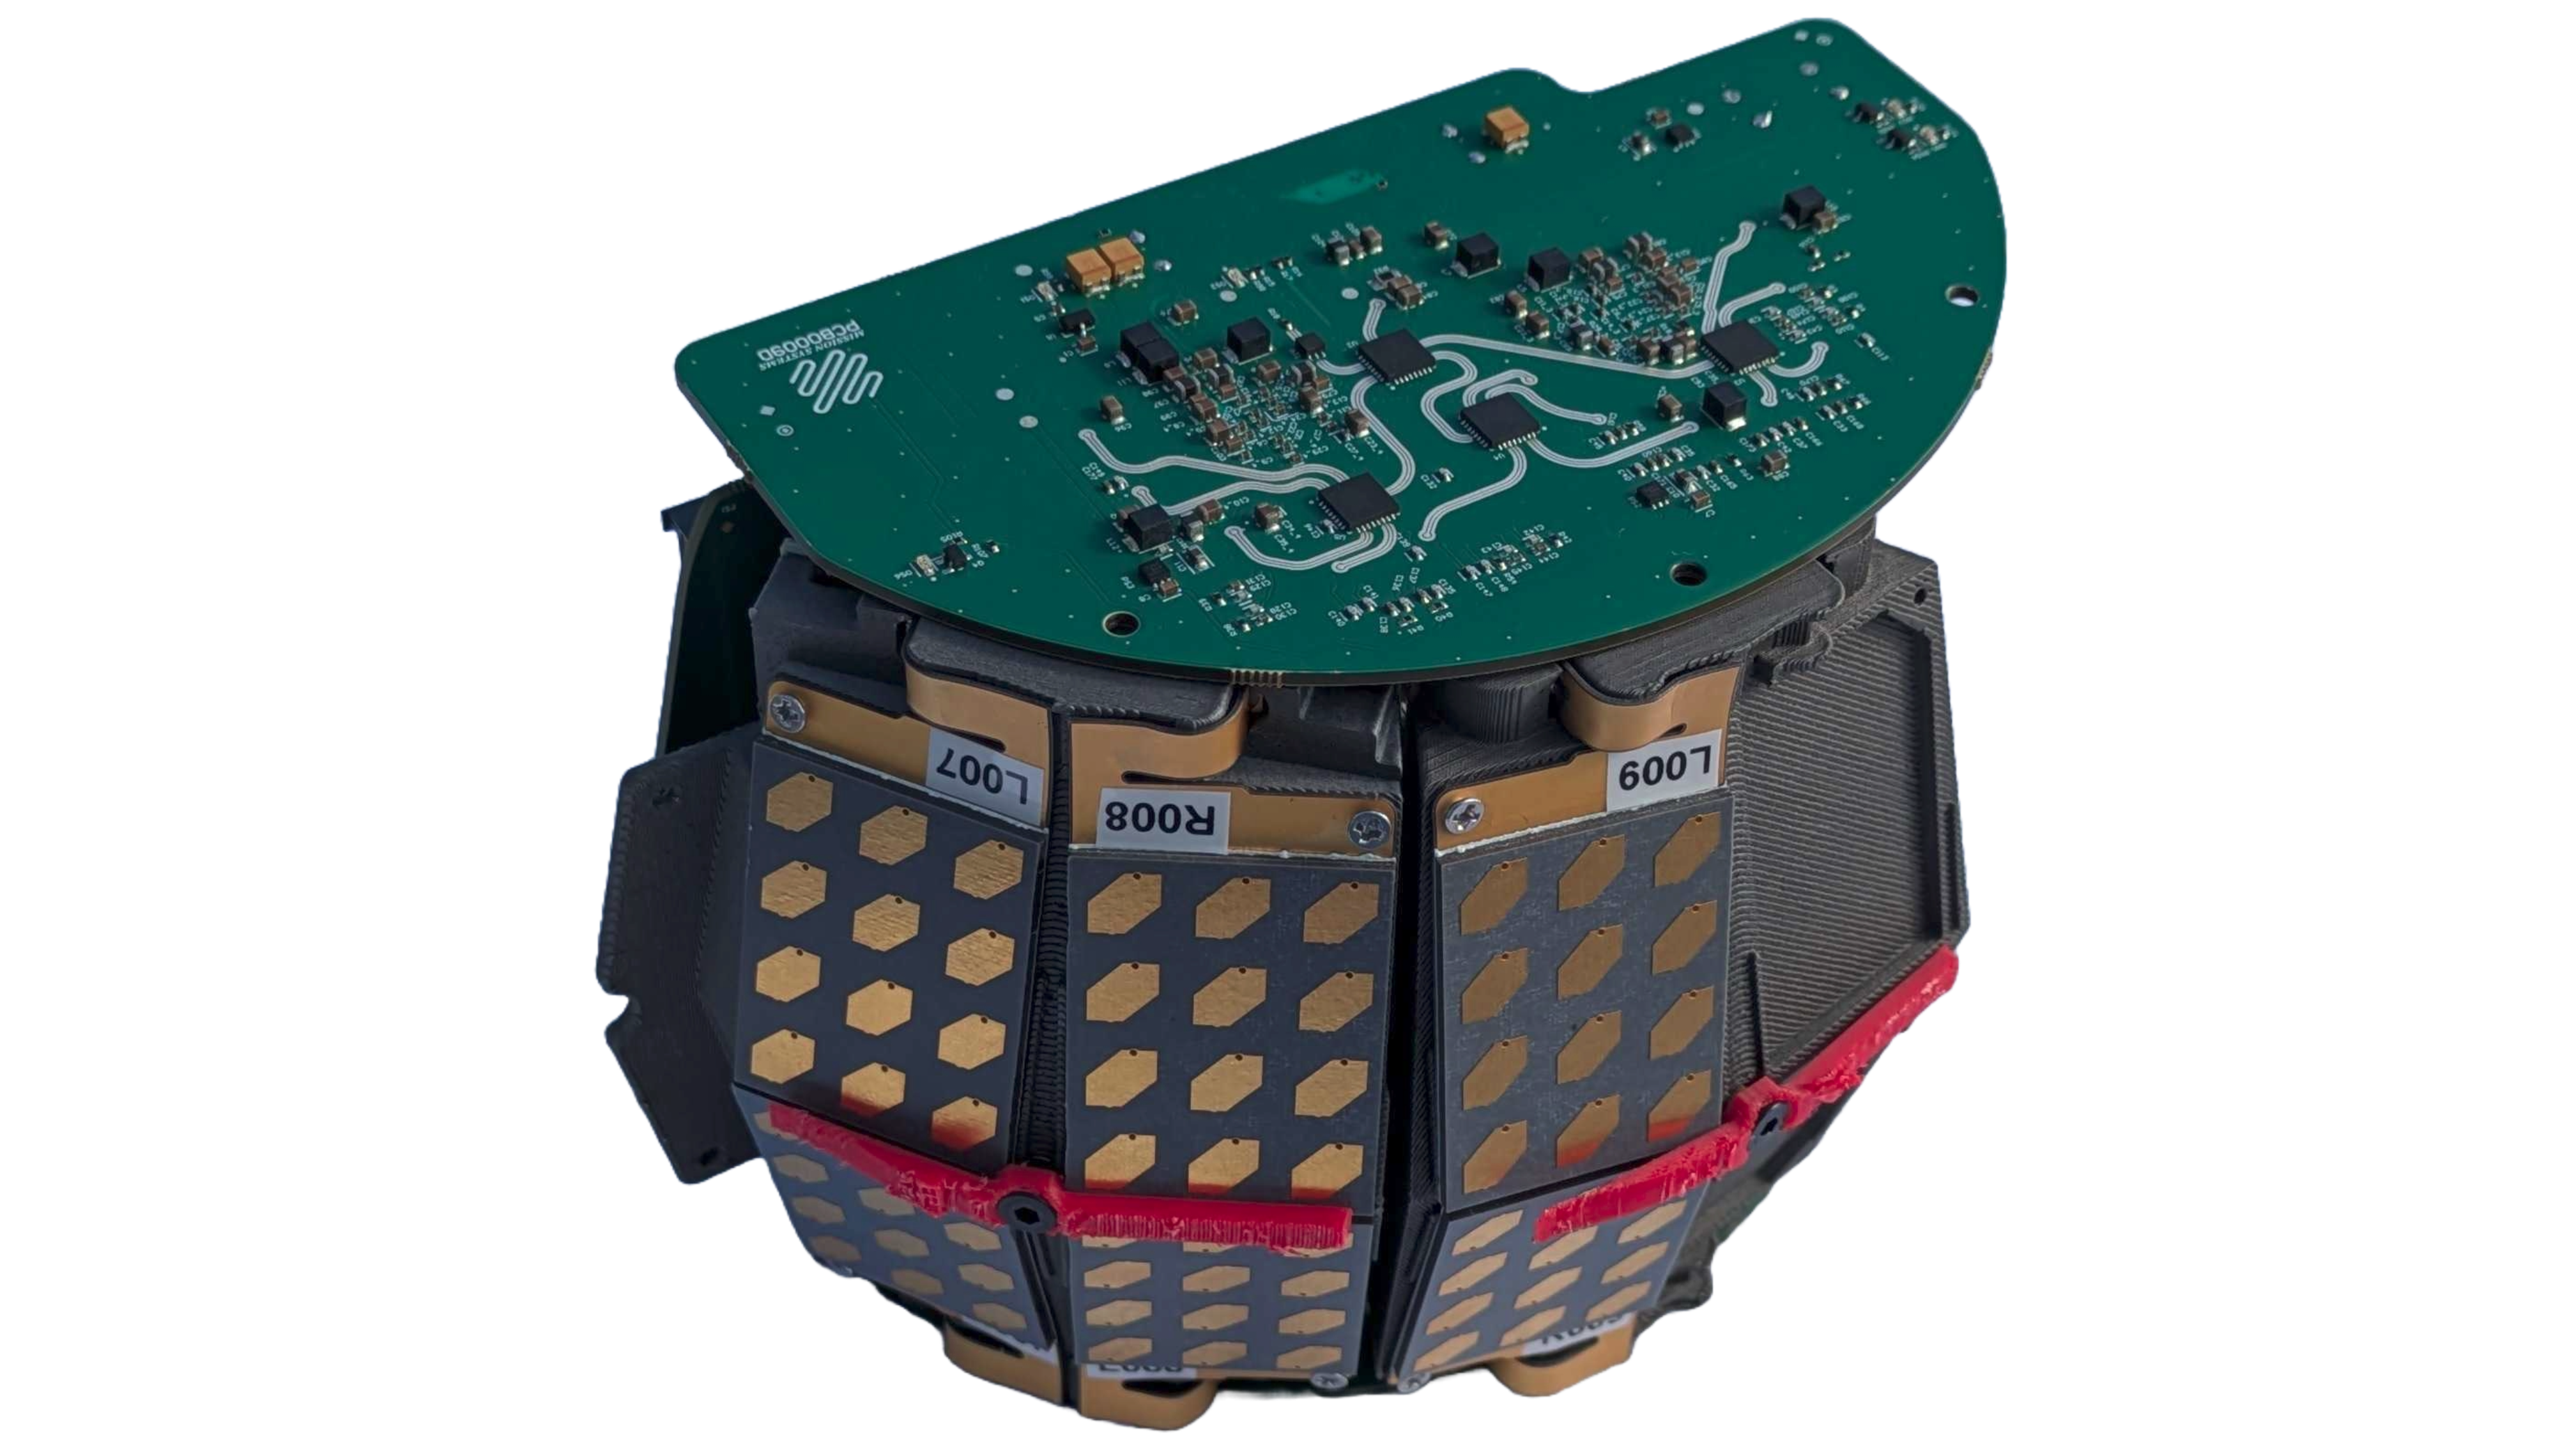
\includegraphics[width=0.7\textwidth]{radar_module.png}
    \caption[Radar Module Photo]{Photo of the radar module with its 6 of its 12 receiver 
    patches arranged in a 3x2 grid.}
    \label{fig:radar-module}
\end{figure}

\begin{figure}[htbp]
    \centering
    \incfig[0.9]{application_level_dataflow} 
    \caption[\small System-level dataflow diagram of the radar pipeline.]{\small System level dataflow diagram. The pre-processing subsystem receives the AWR2243's raw
    radar data over four CSI video streams. The data is organised into frames, each containing many
    chirps. The processing subsystem then outputs
    the data in the form of chirps containing target range information. The aggregator subsystem
    receives the four resulting processed data streams, and combines them into a single data stream
    organised by quadruplets, a collection of four receivers necessary for monopulse angle sensing.
    The detection and tracking subsystem receives a stream of quadruplet chirps, and produces tracks of
    targets in the radar's field of view.}
    \label{fig:system-level-dataflow}
\end{figure}

The methodology is organised into three parts. Firstly, we propose a design of a \mbox{(pre-)processing} 
subsystem that performs formatting, windowing, FFTs, and coherent integration on dense radar data. 
Then, we propose the design of a detection and tracking subsystem that performs CFAR, monopulse angle 
sensing, clustering, and multi-target tracking. Lastly, we describe the datasets used for testing.

\FloatBarrier
\section{Processing Subsystem Evaluation}
\label{sec:processing_app}
The proposed preprocessing subsystem is responsible for receiving the raw radar data from the AWR2242 
radar chips, depicted in Figure \ref{fig:AWR2243},
and preparing the data for detection. An instance of the subsystem runs per incoming video stream. 
Before outputting the data to the aggregator subsystem which is upstream of the detection and 
tracking subsystem. The subsystem performs the following operations sequentially: formatting, windowing, FFT, and 
integration, (see Figure \ref{fig:preprocessing-dataflow}). Below are the implementation and 
experiment details for each of the operations. 

\begin{figure}[htbp]
    \centering
    \incfig[1]{preprocessing_dataflow} 
    \caption[Dataflow for the preprocessing subsystem.]{Dataflow for the preprocessing subsystem. Multiple instances of the subsystem run on
    separate processes, with each instance receiving compressed baseband radar data samples from an
    incoming video stream. Formatting organises samples into contiguous blocks in memory, and discards
    empty chirps. The windowing stage applies a window function to the data to reduce spectral smearing
    in the next stage. The \gls{fft} stage applies a Fourier Transform across fast time into the frequency
    domain, revealing target range. The coherent integration stage sums the complex \gls{fft} values of
    identical pulses within the same frame.} 
    \label{fig:preprocessing-dataflow}
\end{figure}

\begin{figure}
    \centering
    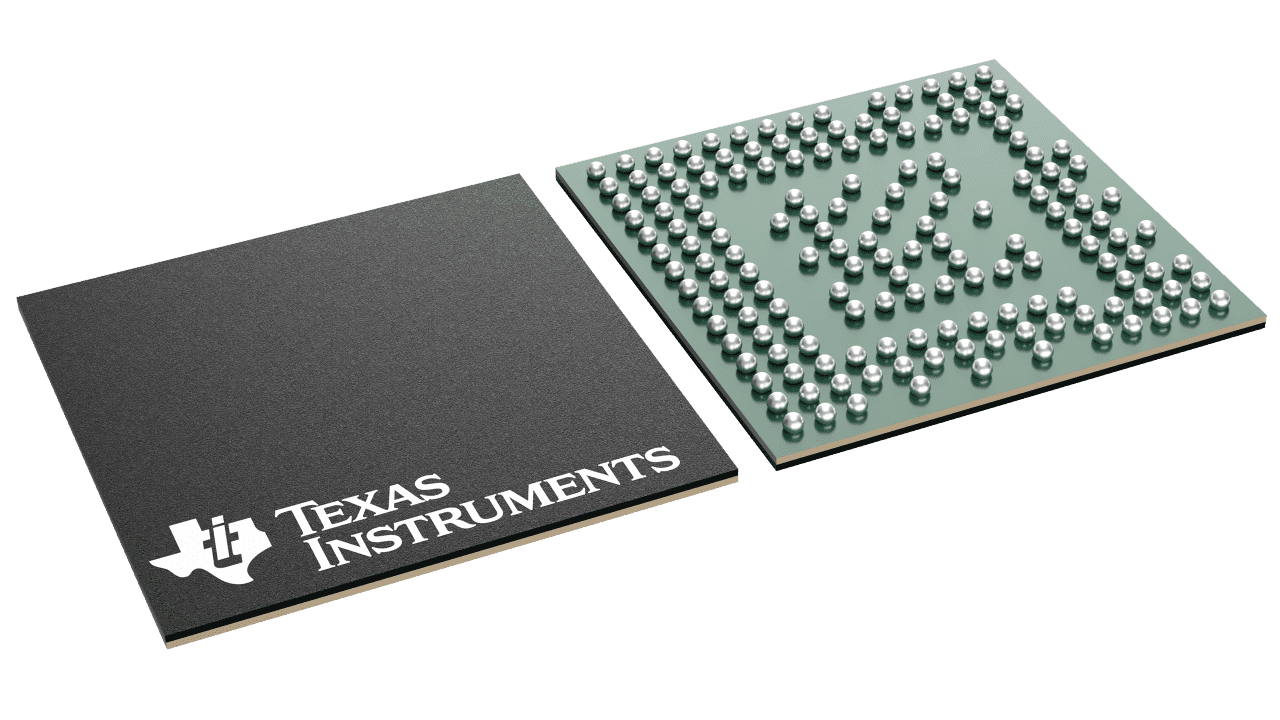
\includegraphics[width=0.5\textwidth]{AWR2243.png}
    \caption[Texas Instruments AWR2243 radar chip.]{Photo of the Texas Instruments AWR2243 radar chip, which is
    used in the radar module. The chip has 3 transmitters and 4 receivers, and outputs the radar data over a CSI
    video stream. The chip is only 10.4mm x 10.4mm, making it suitable for placement on UAV PCBs.}
    \label{fig:AWR2243}
\end{figure}

\subsection{Windowing}
To reveal target range from a single radar pulse, an \gls{fft} is applied to the
de-chirped pulse. 
% The  assumes the finite signal repeats periodically, so when the signal does
% not start and end at the same value, the implicit periodicity introduces a discontinuity. This
% causes energy from a true frequency to spread into adjacent bins — a phenomenon known as spectral
% leakage.

When an \gls{fft} is performed on a finite signal, it is implicitly multiplied by a rectangular window.
A term-wise multiplication in time corresponds to a convolution in the frequency domain, and the
rectangular window's sinc-shaped frequency response has large sidelobes that spread energy from
each frequency bin into its neighbours. By applying a more suitable window function prior to the
FFT, spectral leakage can be reduced, as shown in Figure \ref{fig:hann filter}.

\begin{figure}[htbp]
    \centering
    \includesvg[width=0.6\linewidth]{Images/ffts1}
    \caption[FFT with and without a Hann window showing spectral leakage reduction.]{Results of an \gls{fft} performed on a signal with two frequencies and Gaussian noise, with
    and without a Hann window. Without the Hann window, the bins close to the peak frequency bins 40
    and 45 are significantly elevated due to spectral leakage from those peaks, which would cause
    nearby bins to be falsely detected as targets.}
    \label{fig:hann filter}
\end{figure}

This thesis evaluates a range of practical window functions and their implementation on CPU and GPU. 
Candidate windows include common real-time tapers such as Hann and Hamming, lower-sidelobe windows 
such as Blackman and Blackman--Harris, and adjustable-parameter windows such as Kaiser, which allow 
explicit control over sidelobe level and mainlobe width. Because windowing is a point-wise 
multiplication, it is naturally suited to single instruction, multiple data (SIMD) execution. These 
implementations are compared for their resulting spectral behaviour. 

The sidelobe attenuation and resolution loss are compared for each window and a trade off analysis 
is performed to determine when each window is the most suitable. These procedures provide a basis 
for selecting windows that are spectrally well behaved, sensitive, and 
positively affect the ending track quality. 

\subsection{Integration}
Coherent integration is compared with non coherent integration for their resulting SNR 
improvement, angle estimation quality, and track quality on real and simulated data. 
The relationship between coherent integration window size and the performance metrics 
is also explored. 

After, the latency and throughput of coherent integration is characterised in relation to
the other stages, and the integration window size. The trade off analysis is 
between SNR and latency is performed. The integration stage is also evaluated in the
ablation study of the processing application. 
\section{Detection and Tracking Application Evaluation}
\label{sec:tracking_app}
The proposed detection and tracking subsystem is responsible for receiving the processed 
radar data
across all radar channels from the aggregator subsystem, and producing tracks of
targets in the radar's field of view. The subsystem performs the following operations
sequentially (see Figure \ref{fig:dat-dataflow}): CFAR, clustering, monopulse 
angle sensing, sidelobe suppression (blanking), and multi-target tracking.
Below are the implementation and experiment details for each of the operations.

\begin{figure}[H]
    \centering
    \incfig[1]{detection_and_tracking_dataflow} 
    \caption[Dataflow diagram for the detection and tracking subsystem.]{Dataflow for the detection 
    and tracking subsystem. The subsystem receives the processed radar data across all radar 
    channels from the aggregator subsystem, and produces tracks of targets in the radar's 
    field of view. The subsystem performs the following operations sequentially: CFAR, clustering, 
    monopulse angle sensing, sidelobe suppression (blanking), and multi-target tracking.}
    \label{fig:dat-dataflow}
\end{figure}

\subsection{CFAR}
For finding the CFAR coefficient $\alpha$ (defined in \ref{eqn:threshold}) that gives a desired false 
alarm rate $P_{fa}^{\star}$. The relationship between these variables (Equation 
\ref{eqn:cfar_false_alarm}), cannot be rearranged into a closed-form expression. 

\begin{equation}
    P_{fa}(\alpha;N) = \left( \frac{N}{N+\alpha} \right)^N
    \sum_{k=0}^{3} \binom{N+k-1}{k}
    \left( \frac{\alpha}{N+\alpha} \right)^k
\end{equation}

Since $P_{fa}(\alpha;N)$ is strictly decreasing in $\alpha$, bisection can be used 
to find the value of $\alpha$ that gives the desired false alarm rate \(P_{fa}^{\star}\).

The method begins with $\alpha_{lo}=0$ and increases an upper bound $\alpha_{hi}$ until 
$P_{fa}(\alpha_{hi};N) \leq P_{fa}^{\star}$. It then repeatedly bisects the interval and evaluates 
$P_{fa}(\alpha;N)$ at the midpoint, updating the lower or upper bound depending on whether the resulting 
false alarm rate is above or below the target. This continues until the interval is sufficiently small. 
In this way, $\alpha$ is obtained as the numerical solution that gives the required false alarm rate.

Additionally, three different implementations of CFAR are compared for their latency: a naive
implementation on the CPU, an implementation that uses a prefix sum table, and a naive solution on the
GPU. Additionally, different noise assumptions are tested. The naive implementation involves calculating 
the noise statistic with a repeated sum per sample of interest (see Figure \ref{fig:naive-cfar}). 
The prefix sum table method reduces the 
number of sums required to four per sample of interest regardless of the number of training cells, the
start and end of the left and right window (see 
Figure \ref{fig:prefix-sum-table}). The GPU implementation creates a thread per sample of interest (see 
Figure \ref{fig:gpu-cfar}). A sweep of window size, guard size, frame buffer size and false alarm rate values is 
conducted for each CFAR implementation on real and simulated data. The performance (throughput, latency, 
false alarm rate, sensitivity, and track quality) is compared across configurations in a cost benefit 
analysis. 
This addresses the literature gap in understanding how detection sensitivity and false alarm behaviour 
trade off against latency and throughput under SWaP constraints.

\begin{figure}[!ht]
    \incfig[0.75]{cfar}
    \caption[Naive CPU CFAR implementation.]{Naive Implementation of CFAR for the CPU. Each sample is compared to a threshold
    determined by the power of the samples around it. The threshold is calculated by taking the
    average power of the surrounding samples and multiplying it by a factor \(\alpha\) determined
    by the desired false alarm rate.}
    \label{fig:naive-cfar}
\end{figure}

\begin{figure}[htbp]
    \incfig[0.75]{prefix_sum_table}
    \label{fig:prefix-sum-table}
    \caption[CFAR using a prefix sum table for constant-time noise statistics.]{CFAR implementation using a prefix sum table (cumulative signal power). The prefix sum
    table allows the noise statistic to be calculated with a fixed number of sums per sample of
    interest, regardless of the number of training cells. In this specific case, after the cumulative
    signal power is calculated in processing, it only takes four sums of to find the sum of eight
    training cells.}
\end{figure}

\begin{figure}[htbp]
    \incfig[0.75]{gpu_cfar}
    \label{fig:gpu-cfar}
    \caption[Parallel GPU CFAR implementation.]{CFAR implementation on the GPU. Threads (each depicted as unique colours) are each
    responsible for a sample, allowing for parallel processing of the CFAR algorithm across the entire
    range profile. Each thread calculates its own noise statistic, threshold, and mask.}
\end{figure}

The literature gap regarding algorithmic selection is addressed through an exploration of different CFAR
algorithms, including OS-CFAR, CA-CFAR, SO-CFAR, and GO-CFAR. The effect of these algorithms on detection
sensitivity and track quality is compared. For intuition, Figure \ref{fig:cfar-algorithms} illustrates
the difference in performance of the algorithms on a synthetic signal with 5 peaks. This work 
compares the performance of GO-CFAR, SO-CFAR, and CA-CFAR on simulated data and discusses
the downstream effects of this selection, addressing the literature gap regarding the impact of 
detection algorithms in the noise regimes of miniature radar. Additionally, by analysing the 
performance of both CPU and GPU implementations of CFAR, the literature gap regarding the 
algorithmic implementation under SWaP constraints is addressed. 

\begin{figure}
    \centering
    \incfig[0.81]{cfar_stacked_matched_colours}
    \caption{ Performance of four CFAR variants. Each 
    algorithm registers a detection when its threshold is 
    below the signal. The test signal has 5 peaks that are 
    each surrounded by different noisy distributions. The bottom 
    plot illustrates the detections made by each algorithm. 
    OS-CFAR performs well in this example.}
    \label{fig:cfar-algorithms}
\end{figure}

\subsection{Clustering}
After CFAR occurs, most of the samples (range bins) will be zero. The efficiency loss from 
processing so many zero samples motivates a stage that transforms the detection sparse 
representation into a dense one. Additionally, the widening of the main lobe of each of 
the detections due to the windowing stage creates multiple range bins with detections 
from the same target, which motivates a stage that groups these samples into a single 
detection.
The algorithm that addresses both of these problems, clustering, iterates through the 
range profile, and creates a cluster for each contiguous set of 
detection samples. Then, the complex signals from each of the samples are summed together. 
SNR is expected to improve, as noise will be incoherent within clusters, but the signal
that corresponds to a target will have the same phase across samples, and thus will be 
coherent. The latency of both CPU and GPU implementations of the clustering algorithm 
is measured. Different clustering parameters are tested for their impact on tracking performance, such 
as the allowed gap size between detections.

\subsection{Monopulse Angle Sensing}
Angle sensing converts multi-channel detections into azimuth, elevation and range estimates that 
drive association and tracking. We assess candidate angle discriminators by running controlled 
sweeps over SNR, channel 
imbalance, and multi-target proximity, and measuring angular bias, mean squared error, and confidence. 
The latency and throughput of CPU and GPU implementations are measured. The trade-off involves software implementation details such as warp divergence and instruction-level parallelism. 

The angle sensing algorithm features a few early returns that result in warp divergence on the GPU. 
For example, if the bearing and elevation ratios are outside of the domain over which the polynomial
fit is valid. Instruction level parallelism is a measure of how many instructions can be executed 
in parallel on a single thread. By changing the order of operations, we can potentially increase instruction-level parallelism and reduce the latency of the GPU implementation.

\subsection{Sidelobe Suppression (Blanking)}
When a target exists outside of the field of view of a given radar receiver, the receiver may still
register a detection due to the sidelobes of the antenna pattern. When a target is in the radar's 
field of view, it will land in the main lobe of some receivers and the sidelobes of others (see Figure 
\ref{fig:sidelobes}), resulting
in a strong detection in the correct direction and weaker detections in the wrong directions, all at
the same range. The blanking stage eliminates detections that are likely to be sidelobes by eliminating
detections that are close in range to a stronger detection at the same time step. 

\begin{figure}[htbp]
    \centering
    \begin{minipage}{0.5\textwidth}
        \centering
        \incfig[1]{sidelobes}
        \caption[Sidelobes of the antenna pattern.]{Receivers R1 and R3, which are pointing away from the target,
        still receive significant power from the first sidelobes lining up with the target. }
        \label{fig:sidelobes}
    \end{minipage}
    \begin{minipage}{0.45\textwidth}
        \centering
        \incfig[1]{blanking}
        \caption[Blanking for sidelobe suppression.]{Detections from the sidelobes of R1 and R3 are weaker 
        than R2's detection from the main lobe, and are close in range to R2's detection. R1 and R3's
        detections that are close in range to a stronger detection at the same time step are eliminated.}
        \label{fig:blanking}
    \end{minipage}
\end{figure}

\begin{figure}[htbp]
\end{figure}

The blanking stage will be implemented on the CPU. After clustering and angle sensing, 
the detections come in an ordered list per receiver quadruplet. A CPU implementation would involve,
for each time step, iterating through each of the lists simultaneously and sorting them into one ordered list in O(N) 
time. Then iterating through the ordered list and eliminating detections that are close in range to
a stronger detection. 

% GPU DETAILS BELOW, POTENTIALLY USEFUL
% A GPU implementation would involve creating a thread per detection per quadruplet, 
% performing 3 binary searches to figure out how many detections are nearer than it in range to the radar,
% and mapping itself to the corresponding place in the fully sorted list. In a second pass then, each 
% thread would check the detections near it in the fully sorted list to see if there are any stronger
% detections in range. Since this problem is a standard k-way merge sort, the CUDA Thrust library 
% implementation will be used. This stage can also double as a receiver fusion stage, as detections
% from multiple receivers across different chirps that are close in not just range but also angular 
% position can be merged 
% together. 

\subsection{Multi-Target Tracking}

\begin{figure}[htbp]
    \centering
    \incfig[1]{tracking_dataflow} 
    \caption[Dataflow diagram for the tracking subsystem.]{Dataflow for the tracking stage of the 
    detection and tracking subsystem. Detections are fed into the
    associator of the multi-target tracker, and are then fed into the hypothesiser. 
    The hypothesiser produces a hypothesis per track/detection pair. The associator then 
    finds the optimal assignment
    of detections to tracks. The updater then updates the tracks, and the deleter deletes 
    tracks with poor quality. For the detections that are not associated with any tracks,
    a tentative track is initiated or updated in the initiator, a miniature tracker that
    handles the track initiation and confirmation process. 
    }
    \label{fig:tracking-dataflow}
\end{figure}

The multi-target tracking stage will be implemented entirely on the CPU due to its sequential nature. 
Amplitude based association will be compared to non-amplitude based association for their impact on
track quality. The multi-target tracker has over 20 parameters that can be tuned, and one 
configuration of these parameters will be validated and discussed. Experiments will
be conducted in a variation of SNR, and number of targets, in simulated data. Real 
data will be used to validate the results on static targets. The literature gap regarding the impact
of algorithmic choices in the tracking stage on track quality is addressed through this experiment. 

% EXPLORE MORE
% - Non amplitude based association
% - Amplitude based association
% - ringing 

% \section{Testing Datasets}
% The datasets described below are used for the experiments outlined in the following sections (see Sections \ref{sec:processing_app}, and \ref{sec:tracking_app})
% \begin{itemize}
%     \item \textbf{Generic Sine Waves with Noise}: To validate the correctness of our processing 
%     algorithms as well as their speed, we generate binary files of synthetic radar data consisting of 
%     a complex sine wave with additive white Gaussian noise. This allows us to test the software under 
%     controlled conditions where we can precompute the expected output, and to evaluate the performance 
%     of the software in terms of latency and throughput without the confounding factors of real-world 
%     data. (INCLUDE FIGURE HERE illustrating the signal)  
%     \item \textbf{AWR2243 Recorded Data}: To validate the operation of our pipeline with realistic 
%     data speeds, timing uncertainties, and electrical noise, we record data from our AWR2243 radar 
%     system in TEST\_SOURCE mode. In test source mode, two targets can be simulated on the chip with 
%     position velocity and bounds. The receivers record what the reflected signals from these targets 
%     would look like. While the data recorded is not fully representative of real-world data, it allows 
%     us to test the software with realistic data rates and noise characteristics. 
% \end{itemize}

\section{Testing Datasets}
The datasets described below are used for the experiments outlined in the previous sections 
(\ref{sec:processing_app} and \ref{sec:tracking_app}).

The first dataset is used 
to validate both the correctness and the speed of our processing algorithms during development. 
By generating binary data streams containing complex sine waves with Gaussian noise using bash scripts, 
we can test the radar software under controlled conditions where the expected output can be precomputed 
in advance. This makes it possible to verify algorithmic correctness while also evaluating latency and 
throughput without the additional complexity introduced by real-world phenomena such as multipath 
propagation, data corruption, and non-gaussian noise. An interactive variation of this dataset is 
also used for debugging, allowing the user to adjust parameters such as SNR, range, and bearing/elevation
ratios in real. Figure \ref{fig:synthetic-signal} illustrates an example of a synthetic signal generated 
for testing.

\begin{figure}
    \incfig[0.6]{dataaset1}
    \caption[Example of a synthetic signal generated for testing.]{An 
    example of a synthetic signal generated for testing. The top plot shows the real components of the 
    samples of many received chirps (stacked vertically). Fast time increases to the right and the height 
    of a sample within a chirp is its voltage. In the bottom plot, the horizontal axis is now range, 
    successive chirps are stacked vertically and amplitude is depicted with colour, where yellow is the highest 
    amplitude. 2nd plot is produced by applying an \gls{fft} to each synthetic chirp from the first plot. 
    The transform allow us to visually validate that the frequency to range conversion is correct, 
    and the preprocessing stage is behaving as expected.}
    \label{fig:synthetic-signal}
\end{figure}

The second dataset consists of recorded data from the AWR2243 radar system operating in \verb|TEST_SOURCE| 
mode. This dataset is used to validate the behaviour of the processing pipeline under more realistic 
data rates, timing uncertainties, and electrical noise conditions. In \verb|TEST_SOURCE| mode, the chip can 
simulate two targets with configurable position, velocity, and bounds, and the receivers capture the 
signals that would be reflected from these targets. Although this recorded data is still not fully 
representative of real-world radar returns, it provides a more realistic approximation of practical 
operating conditions than the synthetic sine wave dataset. 
